% \documentclass{beamer}

\documentclass[aspectratio=169, 11pt]{beamer}

\usetheme{Singapore}
% \usepackage{beamerthemesplit}

\setbeamersize{text margin left=2em}  % <- like this
\setbeamersize{text margin right=2em} % <- like this

\usepackage{tabularx}
\usepackage{tikz}
\usetikzlibrary{positioning, fit, arrows.meta}
\usepackage{amsmath,amssymb}

% \setmonofont{Inconsolata}
\usepackage{listings}
\usepackage{color}
\usepackage{xcolor}
\usepackage{algorithm}
\usepackage[noend]{algpseudocode}
\makeatletter
\def\BState{\State\hskip-\ALG@thistlm}
\makeatother
 
\definecolor{codegreen}{rgb}{0,0.6,0}
\definecolor{codegray}{rgb}{0.5,0.5,0.5}
\definecolor{codepurple}{rgb}{0.58,0,0.82}
\definecolor{backcolour}{rgb}{0.95,0.95,0.92}
 
\lstdefinestyle{mystyle}{
    backgroundcolor=\color{backcolour},   
    commentstyle=\color{codegreen},
    keywordstyle=\color{magenta},
    numberstyle=\tiny\color{codegray},
    stringstyle=\color{codepurple},
    basicstyle=\ttfamily\footnotesize,
    breakatwhitespace=true,         
    breaklines=true,                 
    captionpos=b,                    
    keepspaces=true,                 
    numbers=left,                    
    numbersep=5pt,                  
    showspaces=false,                
    showstringspaces=false,
    showtabs=false,                  
    tabsize=2
}
 
\lstset{style=mystyle}
 

\title{Analysis of Neural Language Models for Artificial Data Generation}
\author{Thien Nguyen}
\date{\today}

\begin{document}

% ----------------------------------------------

% title page
\frame{\titlepage}

% % table of contents
% \begin{frame}{Overview}
% \tableofcontents
% \end{frame}
  
% purpose of this iso
\section{Objective} 
\begin{frame}
  \frametitle{Objective}
  \begin{itemize}
    \item Survey the current developments in variational language models.
    \item Implement the VAD.
    \item Compare performances against their earlier counterparts.
  \end{itemize}
\end{frame}

% language models
\section{Literature Survey}
\begin{frame}{Language Models}
    \cite{dyer_conditional_2017} describes an unconditional language model as assigning a probability to a sequence of words,  $w = (w_1, w_2, ..., w_{i-1})$. This probability can be decomposed using the chain rule:

  \begin{align}
    p(w) =& \space p(w_1) \times p(w_2|w_1) \times p(w_3|w_1, w_2) \times ... \times p(w_i|w_1, ..., w_{i-1}) \\
    p(w) =& \prod^{|w|}_{t=1}p(w_t|w_1, ..., w_{t-1}) \\
    p(\boldmath{w}|x) = &{} \prod^{|w|}_{t=1}p(w_t|x,w_1, ..., w_{t-1})
  \end{align}
\end{frame}

% can be done with hidden markov models or naive bayes but the independence assumption limits the expressivity of the language models.

% recurrent networks
\begin{frame}{Recurrent Neural Networks}
  % unrolled diagram
  \begin{figure}[!ht]
    \centering
    \includegraphics[width=100mm]{diagrams/rnn-unrolled.png}
    \caption{RNN and its unrolled form.} 
  \end{figure}
  % equation
  \begin{figure}[!ht]
    \begin{equation}
    \label{eq:rnn}
    \begin{aligned}
      h_t &= tanh(W_{hh}h_{t-1}+W_{xh}x_t)
    \\
    y_t &= W_{hy}h_t
    \end{aligned}
    \end{equation}
    \caption{Equations for the RNN cell.}
  \end{figure}    
\end{frame}

% different types of RNN architectures
\begin{frame}
  \begin{figure}[!ht]
    \centering
    \includegraphics[width=100mm]{diagrams/rnn.jpeg}
    \caption{From left to right: (1) an MLP. (2,3,4,5)  examples of different styles of recurrent neural networks, describing the different types of input and output combinations. (Diagram from \cite{karpathy_unreasonable_2015}). \label{rnn_shapes}} 
  \end{figure}
\end{frame}

% GRUs and LSTMs
\begin{frame}{LSTMs and GRUs}
  % https://www.cc.gatech.edu/~san37/post/dlhc-rnn/
  \begin{figure}[!ht]
    \centering
    \includegraphics[width=100mm]{diagrams/presentation/lstm_gru.png}
  \end{figure}
  % both are designed to circumvent the vanishing/exploding gradients
  % improving long term dependency problems
  % These gated architectures regulate the flow of information coming to and from the cell, helping to mitigate the issue of gradient sensitivity and improving long range dependencies. Gates of the cell are parameterised and therefore learnable.
\end{frame}

% Rectangles represent vectors, with red being the input, blue the output, and green representing the state of the RNNs.
\begin{frame}{Word Embeddings}
  \begin{block}{How do you represent words?}
    \begin{itemize}
      \item You have tens of thousands of words.
      \item How do you mark the relationships between them?
      \item Feeding them into neural networks is not necessarily feasible.
    \end{itemize}
  \end{block}
\end{frame}

\begin{frame}{Word Embeddings}
  \begin{columns}
    % equations on the left
    \begin{column}{0.5\textwidth}
      \begin{itemize}
        \item Converts words to vectors.
        \item Models relationships of words based their co-occurence.
        \item Trained in an unsupervised skip-gram neural network.
      \end{itemize}
    \end{column}
    % diagram on the right
    \begin{column}{0.5\textwidth}
      \begin{figure}[!ht]
        \centering
        \includegraphics[width=80mm]{diagrams/presentation/word2vec_chris.png}
        \end{figure}
    \end{column}
  \end{columns}
\end{frame}


% autoencoders
\begin{frame}{Word Embeddings}
  % A NN that learns a representation of the input data.
  \begin{figure}[!ht]
    \centering
    \includegraphics[width=80mm]{diagrams/presentation/word2vec_example.png}
    \end{figure}
\end{frame}

% autoencoders
\begin{frame}{Autoencoders}
  % A NN that learns a representation of the input data.
  \begin{columns}
    \begin{column}{0.5\textwidth}
      \begin{itemize}
        \item Attempts to faithfully recreate the inputs at the output.
        \item Learns the properties of the input data.
        \item Typically has a layer where its dimension is smaller than the input space - called the latent layer.
      \end{itemize}
    \end{column}
    \begin{column}{0.5\textwidth}
      \begin{figure}[!ht]
        \centering
        \includegraphics[width=75mm]{diagrams/autoencoder.png}
        \end{figure}
    \end{column}
  \end{columns}
\end{frame}

\begin{frame}{Recurrent Language Model - Seq2Seq}
  \begin{figure}
  \centering
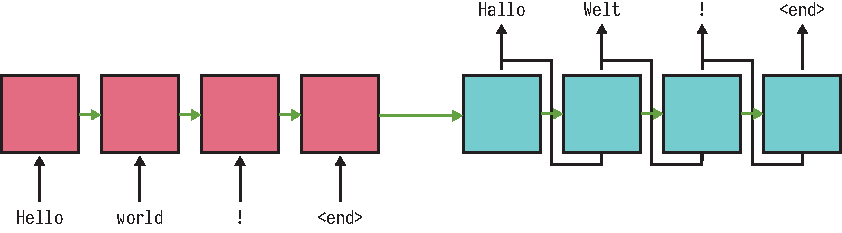
\includegraphics[width=100mm]{diagrams/seq2seq.pdf}
\caption{An abstracted model of the Seq2Seq architecture, where the encoder (pink) takes in the input sequence, and the decoder (blue) shows the output sequence. The encoder outputs are effectively ignored. \label{seq2seq_diagram}}
\end{figure}
\end{frame}

% variational autoencoders
\begin{frame}{Variational Autoencoders}
  \begin{figure}[!ht]
    \centering
    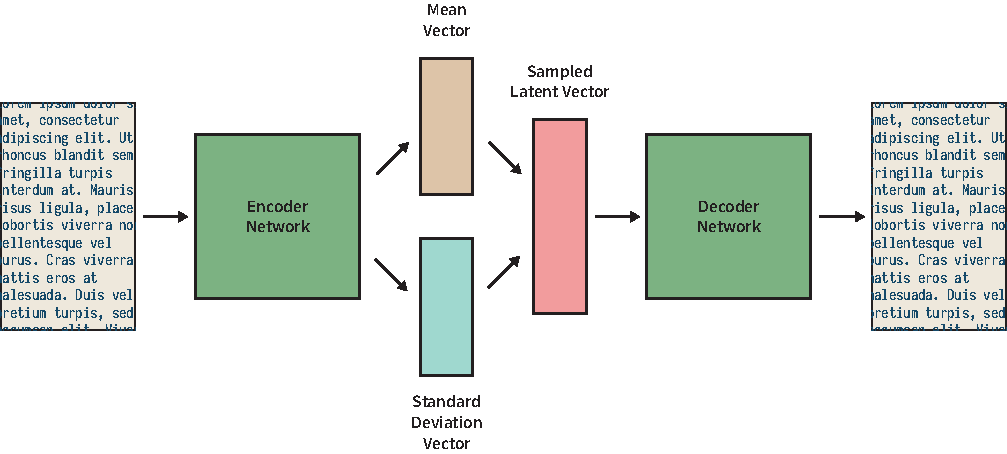
\includegraphics[width=100mm]{diagrams/variational_autoencoders.pdf}
    \caption{An abstracted model architecture for a variational autoencoder, which takes as input some text, and it's predicted output being the same text as the input.\label{vae}}
    \end{figure}
\end{frame}

% elbo
\begin{frame}{\textbf{E}vidence \textbf{L}ower \textbf{Bo}und (ELBO)}
  \begin{equation}
    \label{eqn:elbo}
    \mathcal{L}(\theta, \phi, x, z) = \mathbb{E}_{q \phi (z|x)}[log \thinspace p_{\theta}(x|z)] - D_{KL}(q_{\phi}(z|x)\thinspace||\thinspace p(z)) \leq log (p(x))
  \end{equation}
  \begin{block}{Two Parts:}
    \begin{itemize}
      \item Reconstruction Loss (Smaller is better.)
      \item Distribution divergence (Not actually a loss function - Larger is better!)
    \end{itemize}
  \end{block}
\end{frame}


% variational recurrent langugae model
\begin{frame}{Variational Recurrent Language Model}
  \begin{figure}[!ht]
    \centering
    \includegraphics[width=100mm]{diagrams/seq2seqvae.png}
    \caption{The core structure of the VAE language model - words are represented as embedded vectors (Diagram from \cite{bowman_generating_2015}). \label{vae_seq2seq}}
  \end{figure}

  \begin{itemize}
    \item Does not feed the output as the next input.
    \item Not very useful for conditional response generation.
    \item Good for understanding how to maintain a non-zero KL divergence.
  \end{itemize}
\end{frame}


\begin{frame}{Conditional Variational Recurrent Language Model}
  \begin{figure}[!ht]
    \centering
    \includegraphics[width=100mm]{diagrams/cvae_seq2seq.png}
    \caption{The structure of the CVAE language model. (Diagram from \cite{zhao_learning_2017}). \label{cvae_seq2seq}}
  \end{figure}
\end{frame}

\begin{frame}{Conditional Variational Recurrent Language Model}
  \begin{block}{Recognition and Prior Networks}
    Used to encode posterior and priors.
  \end{block}
  \begin{block}{Bag of Words Loss}
    Mechanism to improve the KL divergence.
  \end{block}
  \begin{block}{Still samples the latent variable once.}
    Considered to reduce expressivity of the responses.
  \end{block}
\end{frame}

% current model
\section{Model Analysis}
\begin{frame}{The Variational Autoregressive Decoder}
  \begin{itemize}
    \item Extension of the CVAE Seq2Seq model.
    \item Utilises \textbf{multi-modal latent sampling}.
    \item Updates the BOW Model.
  \end{itemize}
\end{frame}



\begin{frame}{Decoder}
  \begin{figure}[!ht]
    \centering
    \includegraphics[width=80mm]{diagrams/vad_decoder.png}
    \caption{A High level diagram of the decoding component of the VAD. (Diagram from \cite{du_variational_2018})\label{r:vad_decoder}}
    \end{figure}
\end{frame}

% decoder equations
\begin{frame}{Decoder (Latent Variable)}
  \begin{columns}
    % equations on the left
    \begin{column}{0.5\textwidth}
      \begin{figure}[!ht]
        \begin{equation}
          \begin{split}
            \lbrack \mu^i, \sigma^i \rbrack &=
            f_{infer}([\overrightarrow{h^d_{t-1}}, c_t, \overleftarrow{h^d_t}])
            \\
            q_{\theta}(z_t|\boldsymbol{y}, \boldsymbol{x}) &= \mathcal{N}(\mu^i, \sigma^i) \\
            \lbrack \mu^p, \sigma^p \rbrack &=
            f_{prior}([\overrightarrow{h^d_{t-1}}, c_t])
            \\
            p_{\phi}(z_t|\boldsymbol{y}_{<t}, \boldsymbol{x}) &= \mathcal{N}(\mu^p, \sigma^p)
          \end{split}
        \end{equation}
        \caption{Equations for Inference (left) and Prior (right) models.}
        \label{inf_prior}
        \end{figure}    
    \end{column}
    % diagram on the right
    \begin{column}{0.5\textwidth}  %%<--- here
      \begin{figure}[!ht]
        \centering
        \includegraphics[width=50mm]{diagrams/vad_decoder.png}
        \caption{A High level diagram of the decoding component of the VAD. (Diagram from \cite{du_variational_2018})\label{r:vad_decoder}}
        \end{figure}
    \end{column}
    \end{columns}
  \end{frame}
 

% decoder equations
\begin{frame}{Decoder (Forward RNN)}
  \begin{columns}
    % equations on the left
    \begin{column}{0.5\textwidth}
      \begin{equation}
        \begin{split}
          \overrightarrow{h^d_t} &= \overrightarrow{GRU}([y_{t-1},c_t,z_t], \overrightarrow{h^d_{t-1}}) \\
          p_\phi(y|\boldsymbol{y}_{<t},\boldsymbol{z}_t, \boldsymbol{x}) &= f_{output}([\overrightarrow{h^d_t}, c_t])
        \end{split}
      \end{equation}
    \end{column}
    % diagram on the right
    \begin{column}{0.5\textwidth}  %%<--- here
      \begin{figure}[!ht]
        \centering
        \includegraphics[width=50mm]{diagrams/vad_decoder.png}
        \caption{A High level diagram of the decoding component of the VAD. (Diagram from \cite{du_variational_2018})\label{r:vad_decoder}}
        \end{figure}
    \end{column}
    \end{columns}
  \end{frame}

\begin{frame}{Loss Function}
  \begin{equation}
    \begin{split} 
      \mathcal{L} &= \sum_t [\mathcal{L}_{ELBO}(t) + \alpha \mathcal{L}_{AUX}(t)] \\
      \mathcal{L} &= \sum_t [(\mathcal{L}_{LL}(t) - \mathcal{L}_{KL}(t)) + \alpha \mathcal{L}_{AUX}(t)] 
    \end{split}
  \end{equation}
  \begin{equation}
    \label{eqn:elbo}
    \mathcal{L}_{ELBO}(t) = \mathbb{E}_{q \phi (z|x)}[log \thinspace p_{\theta}(x|z)] - D_{KL}(q_{\phi}(z|x)\thinspace||\thinspace p_\theta(z|x)) \leq log (p(x))
  \end{equation}
  
\end{frame}

% testing
\section{Test Setup}

\subsection{Datasets}
\begin{frame}{Datasets}

  \begin{block}{Penn TreeBank} 
  Model validation dataset. Models would recreate the input sequence.
  \end{block}
  \begin{block}{Open Subtitles} 
  Conditioned sequences. Models would use one subtitle sentence to predict the next sentence.
  \end{block}
  \begin{block}{Amazon Reviews} 
  Conditioned and contextual sequences. Models would use one sentence to predict the next sentence.
  \end{block}
\end{frame}

\subsection{Optimisation Challenges}
\begin{frame}{Optimisation Challenges}
  \begin{block}{KL Collapse}
  AKA Vanishing KL, Posterior Collapse\\
  $D_{KL}(q_{\phi}(z|x)\thinspace||\thinspace p_\theta(z|x)) = 0$
  \end{block}
  \begin{block}{Methods}
  \begin{itemize}
    \item Bag of Words Loss
    \item KL Annealing
    \item Word Dropouts
  \end{itemize}
  \end{block}
  \end{frame}

\subsection{Measurements}
% quantitative measurements
\begin{frame}{Quantitative Measurements}
\small

  \begin{equation*}
    \label{eqn:elbo}
    ELBO = \mathcal{L}(\theta, \phi, x, z) = \mathbb{E}_{q \phi (z|x)}[log \thinspace p_{\theta}(x|z)] - D_{KL}(q_{\phi}(z|x)\thinspace||\thinspace p(z))
  \end{equation*}
  
    \begin{equation*}
      \begin{split}
        BLEU_n = \frac
        {\sum_{S\in C} \sum_{ngram\in S} Count_{clip}(ngram)}
        {\sum_{S\in C} \sum_{ngram\in S} Count(ngram)}
      \end{split}
    % \quad\leftrightarrow\quad
      \quad\quad
      \begin{split}
        ROUGE_n = \frac
        {\sum_{S\in C} \sum_{ngram\in S} Count_{matched}(ngram)}
        {\sum_{S\in C} \sum_{ngram\in S} Count(ngram)}
      \end{split}
    \end{equation*}


    \begin{equation*}
      f1_{n} = 2 \cdot \frac{BLEU_n \cdot ROUGE_n}{BLEU_n + ROUGE_n}
    \end{equation*}

\end{frame}

% semantic variance
\begin{frame}{Semantic Variance}

    \begin{algorithmic}[1]
    \Procedure{Semantic Variance}{}
  
    \State $\textit{query} \gets \text{input }\textit{sequence}$
    \State $\textit{resp} \gets \text{[]}$
    
  
    \For{\textit{i} $=1$ to $n$ } 
      \State $r_i \gets \text{model(}\textit{query}\text{)}$
      \State $r_i \gets \text{[}\text{embedding}\text{(} token \text{) for } token $\emph{ in }$r_i$\text{]}
      % \State $r_i \gets \textit{mean}\text{(}r_i\text{)}$
      \State $\textit{resp}\text{[}\textit{i}\text{]} \gets \textit{mean}\text{(}r_i\text{)}$
    \EndFor 
  
    \State \emph{m} $\gets \textit{mean} \text{(} \textit{resp} \text{)}$
  
    \State \Return $\textit{max}\text{(}\textit{euclidean}\text{(}m, r_{i=1 \text{ to } n}\text{))}$
    \EndProcedure
    \end{algorithmic}

\end{frame}

% results
\section{Results}

\subsection{Quantitative Measurements}
\begin{frame}{ELBO: Reconstruction Loss}
  \begin{figure}[!ht]
    \centering
    \includegraphics[width=130mm]{results/nll.pdf}
    \caption{Reconstruction losses of the three models across the three datasets; lower loss is better. \label{r:nll}}
    \end{figure}
\end{frame}

\begin{frame}{ELBO: KL Ratio}
  \begin{figure}[!ht]
    \centering
    \includegraphics[width=130mm]{results/kl_ratio.pdf}
    \caption{KL ratios of the three models across the three datasets; higher is better.\label{r:kl_ratio}}
    \end{figure}
\end{frame}

\begin{frame}{BLEU}
  \begin{figure}[!ht]
    \centering
    \includegraphics[width=130mm]{results/bleu1.pdf}
    \caption{BLEU\textsubscript{1} scores of the three models across the three datasets; higher is better.\label{r:bleu}}
    \end{figure}  
\end{frame}

\begin{frame}{ROUGE}
  \begin{figure}[!ht]
    \centering
    \includegraphics[width=130mm]{results/rouge_1.pdf}
    \caption{ROUGE\textsubscript{1} scores of the three models across the three datasets; higher is better.\label{r:rouge}}
    \end{figure}  
\end{frame}

\begin{frame}{F1}
  \begin{figure}[!ht]
    \centering
    \includegraphics[width=130mm]{results/f1.pdf}
    \caption{F1\textsubscript{1-gram} scores across the three models; higher is better.\label{r:f1}}
    \end{figure}
\end{frame}

\begin{frame}{Semantic Similarity}
  \begin{figure}[!ht]
    \centering
    \includegraphics[width=130mm]{results/semantic_similarity.pdf}
    \caption{Semantic similarity scores across the datasets and models, higher is more varied.\label{r:variance}}
    \end{figure}
\end{frame}
% examples

\subsection{Generated Examples}
% penn
\begin{frame}{Generated Examples - Penn TreeBank}
  \small
  \begin{columns}
    % left
    \begin{column}{0.5\textwidth}

        these stocks eventually reopened 

      \noindent\rule{\textwidth}{0.4pt}
      \begin{block}{Bowman}
        the  \textless{}unk\textgreater\space \$ cents \textless{}unk\textgreater\space the \textless{}unk\textgreater\space  open      
      \end{block}
      \begin{block}{Seq2Seq}
        these stocks eventually reopened 
      \end{block}
      \begin{block}{VAD}
        these stocks eventually reopened 
      \end{block}
    \end{column}
    % right
    \begin{column}{0.5\textwidth}
     
        as a result the link between the futures and stock markets , apart   
  
      \noindent\rule{\textwidth}{0.4pt}
      \begin{block}{Bowman}
        they is n't elaborate whether the \textless{}unk\textgreater\space  is a we is s going to be a a years
      \end{block}
      \begin{block}{Seq2Seq}
        as a result the link between the futures and stock markets , apart 
      \end{block}
      \begin{block}{VAD}
        as a result the link between the futures between and futures markets apart
      \end{block}
    \end{column}
  \end{columns}
\end{frame}

% subtitles
\begin{frame}{Generated Examples - Open Subtitles}
  \small
  \begin{columns}
    % left
    \begin{column}{0.5\textwidth}
      i give you ride.
      \noindent\rule{\textwidth}{0.4pt}
      \begin{block}{Bowman}
        N/A 
      \end{block}
      \begin{block}{Seq2Seq}
        you ' re going to take a delivery hour
      \end{block}
      \begin{block}{VAD}
        i ' m gon na take a walk . 
      \end{block}
    \end{column}
    % right
    \begin{column}{0.5\textwidth}
      not exactly.
      \noindent\rule{\textwidth}{0.4pt}
      \begin{block}{Bowman}
        ?
      \end{block}
      \begin{block}{Seq2Seq}
        he ' s hideous \textless{}unk\textgreater\space ,  he ' s a musician
      \end{block}
      \begin{block}{VAD}
        i ' m gon na be able to finish the door . 
      \end{block}
    \end{column}
  \end{columns}
\end{frame}

% amazon
\begin{frame}{Generated Examples - Amazon Reviews}
  \begin{columns}
    % left
    \begin{column}{0.5\textwidth}
      b 0 0 d q d c 1 y 6 rating\_4.0 polarity\_0.8 i also have a background in it .   
      \noindent\rule{\textwidth}{0.4pt}
      \begin{block}{Bowman}
        i the : the the the , you 's the i , is the ,             
      \end{block}
      \begin{block}{Seq2Seq}
        i am going to get it to work well .    
      \end{block}
      \begin{block}{VAD}
        the email has a nice connection .    
      \end{block}
    \end{column}
    % right
    \begin{column}{0.5\textwidth}
        b 0 0 9 l l 9 v d g rating\_5.0 polarity\_-0.8 you will need the desktop to run larger things off of , and to use a printer remotely .
      \noindent\rule{\textwidth}{0.4pt}
      \begin{block}{Bowman}
        N/A
      \end{block}
      \begin{block}{Seq2Seq}
        i have a fit of the canon . 
      \end{block}
      \begin{block}{VAD}
        i a little to in distracting for the price .
      \end{block}
    \end{column}
  \end{columns}
\end{frame}

% demo
\begin{frame}
  \begin{block}{Demo}
    Source code: https://github.com/thien/iso
  \end{block}
\end{frame}

\section{Evaluation}
\begin{frame}{Evaluation}
  \begin{block}{Amazon performance is below expectations}
    Could be attributed to a variety of factors, ranging from data sanitisation, to contextual conditioning, to inappropiate word embeddings.
  \end{block}
  \begin{block}{Dataset sizes were handicapped}
    Caused by computational constraints.
  \end{block}
  \begin{block}{Spurious SBOW $\alpha$ weights}
    Attempts to contact the original authors of the VAD regarding missing information has been unsuccessful.
  \end{block}
\end{frame}

% conclusion
\section{Conclusion}
\begin{frame}{Conclusion}
  \begin{block}{It is possible!}
    The VAD has shown to express variety in responses, greater so than the VAD and the Seq2Seq models.
  \end{block}
  \begin{block}{Performance could be improved}
    The amazon dataset could be better augmented to improve VAD performance.
  \end{block}
  \begin{block}{Future Work}
    Experimentation on the SBOW, Augmentation for an Adversarial approach.
  \end{block}
  
\end{frame} 


\section*{References}
\begin{frame}[allowframebreaks]
  \frametitle{References} 
  \small
  \bibliographystyle{apalike}
  \bibliography{ref} 
\end{frame}

\end{document}